\section{Arquitectura del sistema} 

En la Figura \ref{arq_sistema} se muestra una visión de la arquitectura del sistema. Se
trata de una arquitectura cliente-servidor a través de RMI. El cliente usa
un proxy para comunicarse con el servidor y éste conoce un proxy de cada
cliente con el que se comunica. Toda la logica del juego reside en el cliente.

 \begin{figure}[h]
 \centering
 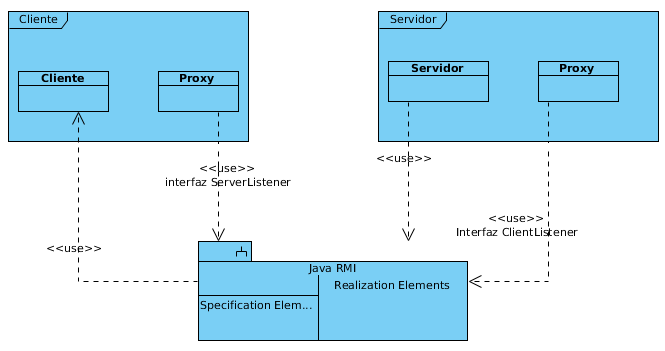
\includegraphics[scale=0.65]{img/arquitectura/arquitectura.png}
 \caption{Arquitectura del sistema}
 \label{arq_sistema}
 \end{figure}

\subsection{Arquitectura del cliente}
 
En la Figura \ref{arq_cliente} se muestra la arquitectura del cliente. Se ha utilizado una arquitectura MVC.
Además, se incluye una capa de comunicación:

\begin{itemize}
 \item \emph{Presentación:} Contiene las clases de las ventanas que se muestran al usuario y las interfaces que implementan.
 \item \emph{Controlador:} Contiene la lógica de control. Se encarga de comunicar a la interfaz los cambios de estado de la
 capa de dominio y de modificar el estado del dominio atendiendo a los cambios en la interfaz del juego.
 \item \emph{Dominio:} Contiene toda la lógica del juego. La clase Tablero9x9 es la clase principal e implementa las reglas del 
 juego. Se utiliza el patrón fachada para obtener un punto de acceso único a la capa de dominio. La clase encargada de 
 esta abstracción es FTERD.
 \item \emph{Comunicación:} Contiene las clases que realizan la función de \emph{listener} como es el caso de la clase Cliente,
 y el proxy con el servidor. Estas clases solamente se encargan del envío de los respectivos mensajes al servidor o a la fachada
 del paquete de dominio.
\end{itemize}

 \begin{figure}[h]
 \centering
 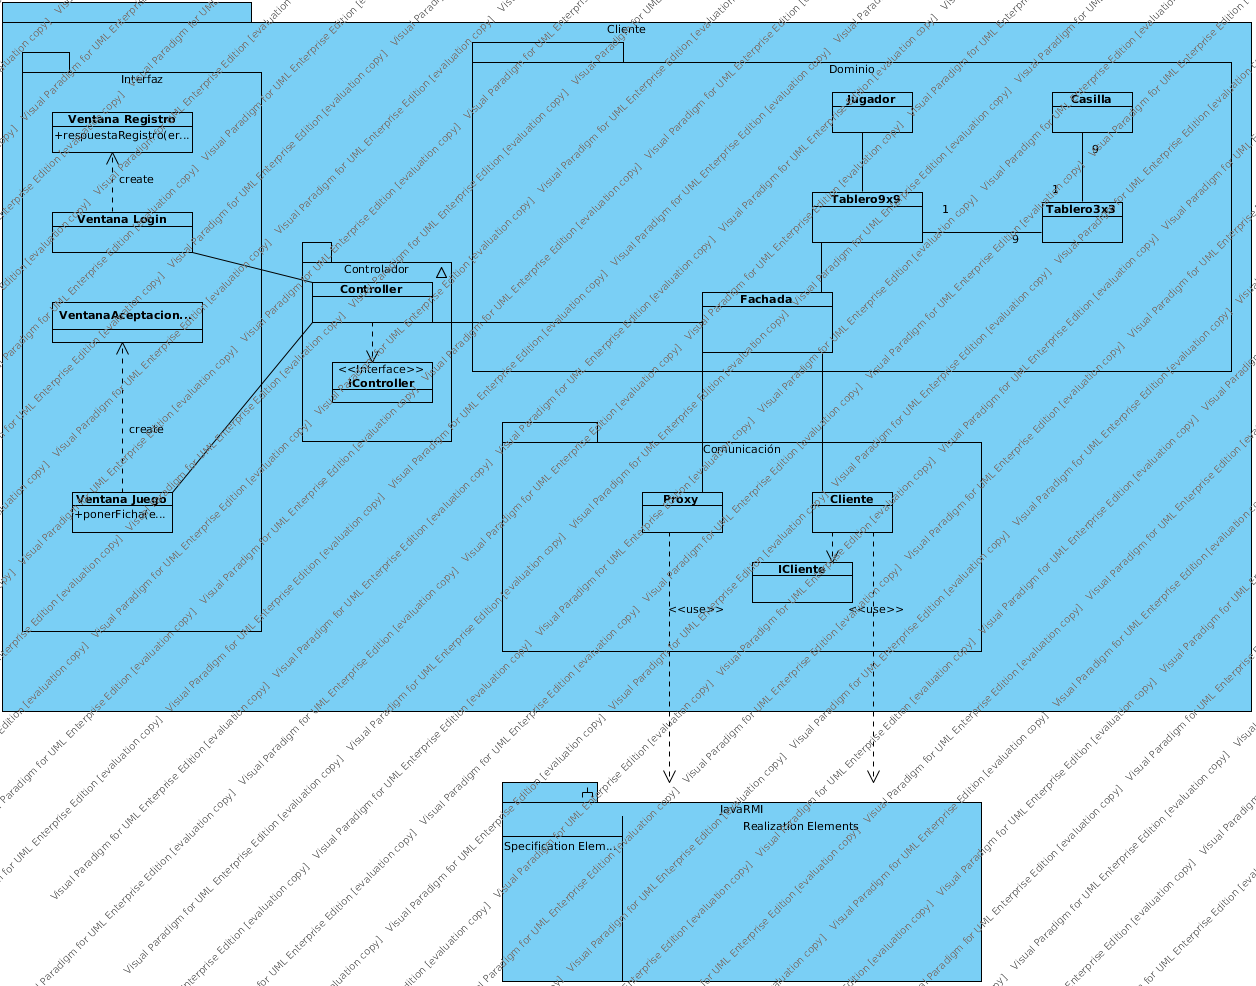
\includegraphics[scale=0.4]{img/arq_Cliente.png}
 \caption{Arquitectura del cliente}
 \label{arq_cliente}
 \end{figure}

\subsection{Arquitectura del servidor}

En la Figura \ref{arq_servidor} se muestra la arquitectura multicapa del servidor:

\begin{itemize}
 \item \emph{Comunicación:} Contiene las clases encargadas de la comunicación, en este caso la clase servidor y su interfaz
 RMI. La clase servidor actúa como \emph{listener} para escuchar solicitudes de los clientes. También responde a esos clientes,
 ya que internamente guarda una hash con los clientes que se han dado de alta en el sistema.
 \item \emph{Persistencia:} Contiene las clases encargadas de almacenar las partidas y sus respectivos tableros, jugadores
 y movimientos. Entre esas clases está la base \emph{Broker}, que actúa como agente entre el subsistema de base de datos y
 el sistema del servidor. Se ha optado por utilizar un patrón de fabricación pura en lugar de seguir el patrón experto para
 la persistencia. De esta forma, un conjunto de clases \emph{DAO} especializadas se encargan de almacenar los diferentes
 aspectos del dominio.
 \item \emph{Dominio:} Contiene las clases de dominio como las encargadas de representar a cualquier juego, además de la
 clase Fachada. Esta clase contiene una referencia a cada uno de los modelos que se están jugando en el sistema, es decir,
 contiene todos los tableros activos.
\end{itemize}


 \begin{figure}[h]
 \centering
 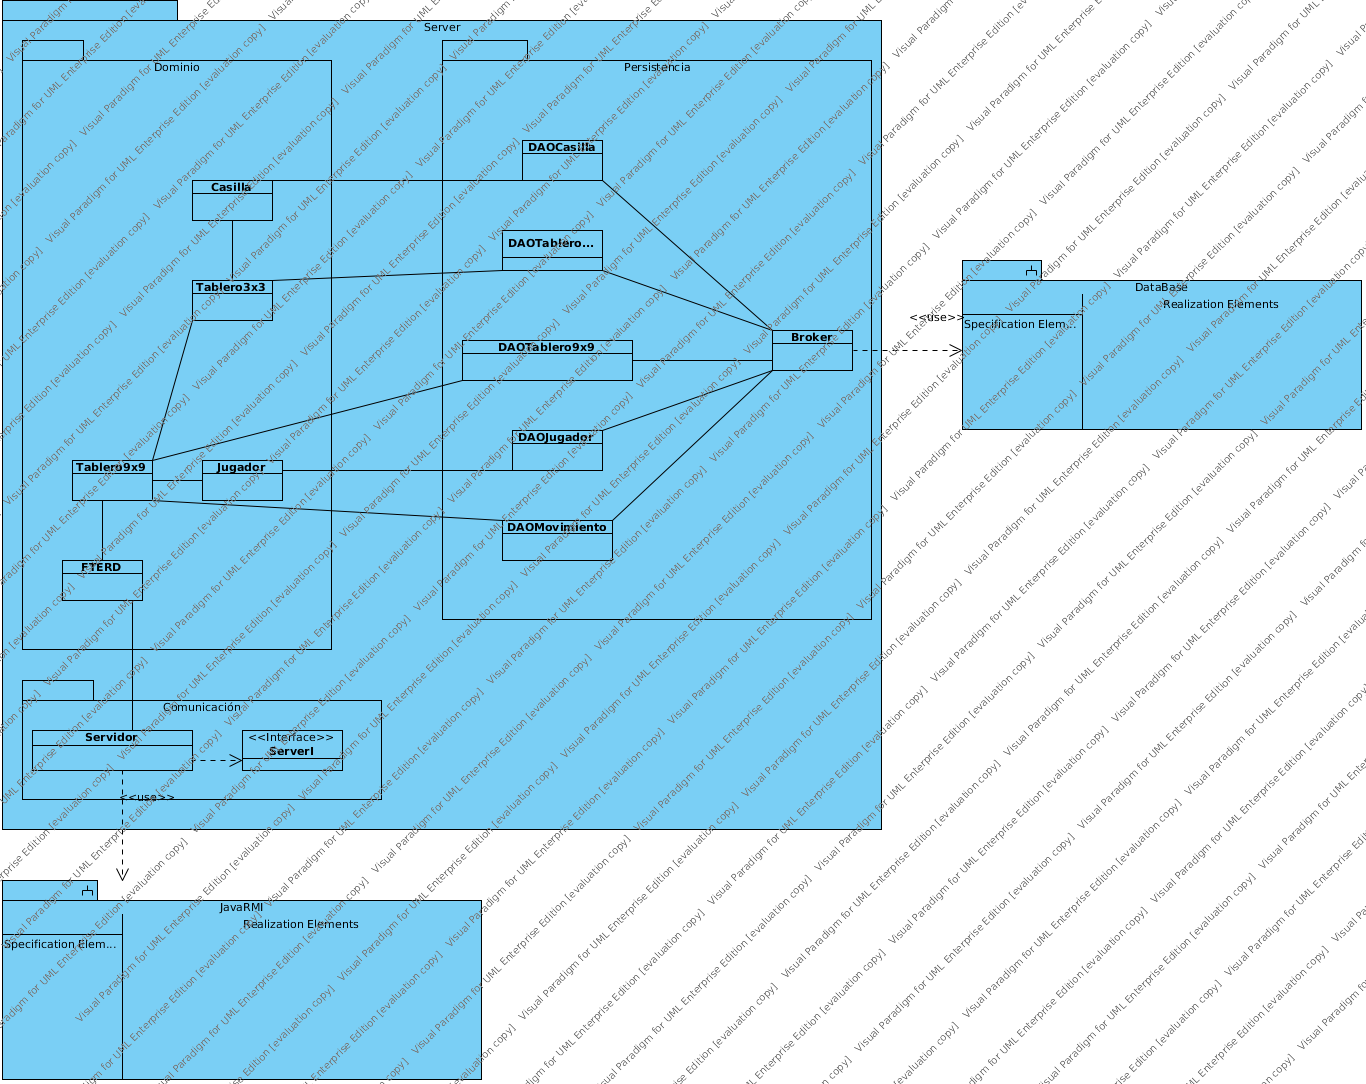
\includegraphics[scale=0.4]{img/arq_Servidor.png}
 \caption{Arquitectura del servidor}
 \label{arq_servidor}
 \end{figure}
 